\documentclass[10pt]{amsart}

\usepackage{tikz}
\usetikzlibrary{quantikz}
\usepackage[utf8]{inputenc}
\usepackage{subcaption}
\usepackage{bm}
\usepackage{amsmath, amsfonts, hyperref,braket,amssymb}
% Define theorem-like environments with independent numbering
\newtheorem{theorem}{Theorem}
\newtheorem{lemma}{Lemma}
\newtheorem{conjecture}{Conjecture}
\newtheorem{definition}{Definition}
\newtheorem{example}{Example}
\newtheorem{proposition}{Proposition}
\newtheorem{corollary}{Corollary}
\newcommand{\A}{\mathcal{A}} 
\newcommand{\E}{\mathcal{E}}
\newcommand{\XX}{\chi}
\newcommand{\X}{\textbf{X}}


\newcommand{\dmat}[1]{{| #1 \rangle \langle #1 |}} 

\newcommand{\rl}[1]{{\rangle \langle}} 
\newcommand{\dm}[2]{\left|#1\right\rangle\left\langle#2\right|}

\newcommand{\EE}{{\mathcal E}}



\DeclareMathOperator{\Tr}{\textnormal{Tr}}


\title[Quantum algorithm for preparing microcanonical ensembles]{Quantum algorithm for \\ preparing microcanonical ensembles}
\author{Oli, Subhayan}
\begin{document}
\maketitle

\begin{abstract}
    We illustrate an algorithmic framework for sampling from a microcanonical ensemble of a given Hamiltonian on a quantum computer. By iteratively applying a dissipative map we drive the state vector into a desired eigenspace. %through a sequence of projectors parametrised by their schedules. 
    %, that drives any state to an state in the eigenspace within a given energy interval. 
    We give a scalable quantum circuit used for each iteration and prove  finite time convergence of this algorithm under idealised setting. 
    We then report a proof-of-concept demonstration of the method on a publicly available IBM-Q device.
    We then numerically study convergence rates of the algorithm to sample microcanonical ensembles of Kitaev model. We finally present a conjecture about the complexity of this method.   
\end{abstract}


%Framework using integral transformations on operators

%The algorithm is an iterative sequence of quantum circuits. Each quantum circuit implements a map. The map implements a spectral projection, to filter eigenstates. 
%Definition of the problem

% Motivation why this is interesting - microcannonical ensembles.

% Intuitions

% Related Works,

% Notation



\subsection*{Notation}
% integral transformation on operators 
% e.g., operator fourier transformations. 
% e.g., kickflip transformations
A quantum state $\rho$ is a positive semidefinite operator on Hilbert space $\mathcal{H}$, with trace one. 
A Hamiltonian $H$ on $n$ qubits is a $D=(\mathbb{C}^2)^{\otimes n}$ dimensional Hermitian operator. A Hamiltonian $H$ is said to be \textit{k-local} if it can be written as $H=\sum_{j} H_j$, such that each $H_j$ acts non-trivially only on atmost $k$ qubits.\\
For a Hamiltonian, $H$, denote $H \cong \sum_{j} \lambda_j \dmat{\phi_j}$ be the spectral decomposition. %For a finite interval $\Lambda = [\Lambda_0,\Lambda_1]$, let $\Theta_{\Lambda}^{(H)}$ be the set of states spanned by the eigenvectors of $H$ with eigenvalues in $\Lambda$, and write $\Theta_{\Lambda}= \text{span}\{ \dm{\phi_j}{\phi_k} : H \ket{\phi_j} = \lambda_j \ket{\phi_j}, H \ket{\phi_k} = \lambda_k \ket{\phi_k}, \text{ and } \lambda_j,\lambda_k \in \Lambda \}$. \\
We will assume throughout that inputs are given as a finite bitstring of length $N$. %We call an algorithm to be efficient/scalable if the resources required to solve the problem instance scales polynomially in the number of bits required to describe the problem.
%% Should we say what is a quantum algorithm?
%A quantum algorithm on n qubits is a sequence of gates, given as $SU(4)\times [n]$,  unitary transform. 
Let $\dm{1}{0} = \begin{bmatrix}
    0 & 0  \\ 1 & 0
\end{bmatrix}$. 

\section{Introduction}


\begin{definition}[Microcanonical Ensemble] 
For bounded norm Hamiltonian $H$ and interval $\Lambda=[\Lambda_0,\Lambda_1]$, the microcanonical ensemble $\Theta^{(H)}_{\Lambda}$ is the set of quantum states spanned by eigenstates of $H \cong \sum_j\lambda_j \dmat{\phi_j} $ with eigenvalues, $\lambda_j \in \Lambda$, and write $\Theta_{\Lambda}= \text{span}\{ \dm{\phi_j}{\phi_k} : H \ket{\phi_j} = \lambda_j \ket{\phi_j}, H \ket{\phi_k} = \lambda_k \ket{\phi_k}, \text{ and } \lambda_j,\lambda_k \in \Lambda \}$. \\ 
\end{definition}



We describe here a idealised quantum algorithm for sampling microcanonical ensembles, given a Hamiltonian $H_S$ and interval $\Lambda = [\Lambda_0,\Lambda_1]$. The proposed algorithm iteratively applies a map,  $\E_\X: \rho_k \rightarrow \rho_{k+1}$ (defined in \eqref{eq_map}), that projects a state vector $\rho_k$ into stable subspace $\Theta_{\Lambda}$, which acts as a sink. We show that finitely many repeated applications of generic $\E_\X$ on any input state then prepares a quantum state that has large overlap with the microcanonical ensemble, with high probability and prove the following propositions in theorems \ref{theorem_finite_convergence_ideal} and \ref{theorem_finite_convergence_noisy}

\newpage
\begin{proposition}
    Given a $n$ qubit Hamiltonian $H_s \cong \sum_{j=1}^{2^n}\lambda_j\dmat{\phi_j}$ and an finite interval $\Lambda$, and a parameter $\epsilon>0$, generic maps $\E_\X^{\Lambda}$ satisfy the following, 
    
    \begin{enumerate}
        \item There exists a finite $r$ such that repeatedly applying generic $\E_\X^{\Lambda}$
    $r$ times to any initial quantum state $\rho_0$ synthesises a state $\rho_r = (\E_\X^{\Lambda})^r(\rho_0)$ that is almost fully supported by the microcanonical ensemble as in Theorem \ref{theorem_finite_convergence_ideal}:
    $$
\mathbb{E}_X \sum_{j: \lambda_j \in \Lambda} \braket{\phi_j | \rho_r | \phi_j} \geq 1 - \varepsilon.$$
 
    \item The above holds also when $\E_\X^{\Lambda}$ is approximated by a quantum circuit upto $\epsilon< \frac{1}{N}$ precision wrt some matrix norm  [as in Theorem \ref{theorem_finite_convergence_noisy}]     
    \item There exists a quantum circuit implementing the map $\mathcal{E}_X$ upto $\epsilon$. 
        \end{enumerate}
\end{proposition}
\textcolor{orange}{Can we formalise and say if the rate of convergence is exponentially fast in the ideal case? }

This algorithmic framework extends ideas previously described in context of preparing ground states \cite{} and Gibbs ensembles \cite{} using dissipative methods \cite{}. We using a combination of techniques relating to operator Fourier transformations \cite{}, signal processing\cite{}, and quadrature rules \cite{}. Similar algorithmic frameworks have been proposed in context of algorithmic cooling \cite{} and quantum collision models \cite{}. 


In contrast to the previous approaches, this article aims to give a self-contained exposition of the algorithm and prove finite time convergence from first principles, without explicitly using GKLS equations \cite{}. GKLS equations generalise the Redfield and Davies equations and describe dynamics on open quantum systems as a completely positive map on positive semidefinite operators. These constructions use the Born-Oppenheimer approximation, secular approximation (rotative-wave approximations), Markov assumptions, which typically assume coupling with a infinite dimensional bath environment. However following from Stienspring-Naimark dilation theorems \cite{}, one may intuit that these assumptions can be relaxed for algorithmic context. We are able to circumvent assumptions and able to obtain an exact form of the dynamics for our state update in Lemma \ref{lemma_simplify_h}. 

Several similar works assume the validity of  eigenstate thermalisation hypothesis (ETH) for all eigenstates \cite{} to argue polynomial time convergence for ground state and Gibbs state ensembles \cite{}, which is more impressive than finite time convergence. However, as many of these works rightfully also point out, while ETH assumption may be a good heuristic \cite{}, it may fail to hold in certain regimes.  In our approach we are able to simply the analysis by instead using k-designs that approximate the first k moments of the haar random distribution. 


We report the efficacy of the method on certain toy models such as Real diagonal matrices, TFIM model, and Heisenberg model in sections \cite{} that optimistically suggest an exponentially fast rate of convergence and complexity growing polynomially in the number of qubits and logarithmically in density of states. We make use of readily available numerical integration techniques and Baker-Cambell-Hausdorff expansion to give a Hamiltonian to Circuit map to approximating the map $\E_\X$.  

Our work however shares similar shortcoming as the previous approaches involving operator fourier transformations, in the sense that the circuit description given here is of \textcolor{orange}{exponential depth}. This can however be further improved in future works. We observe that preparing a microcanonical ensemble is atleast as hard as preparing a ground state in section [], and show the problem of preparing a state in a microcanonical ensembles for k-local Hamiltonians is QMA-hard. 

%should we also define a probability measure on these ensembles? e.g. gibbs ensemble is a probability measure as exp(bx) and ground state is a a delta function.

\newpage

\section{Algorithmic Framework}
Given a particular Hamiltonian $H_s$ with eigenstates $\ket{\phi_i}$ and eigenvalues $\lambda_i$, the spectral sieve algorithm is an iterative algorithm that allows us to drive an initial state $\rho_0 = \sum_{jk} p_{i,j} \ket{ \phi_j }\bra{\phi_k}$ into the subspace $\Theta_{\Lambda} = \text{span}(\{ \ket{\phi_j}\bra{\phi_k} \}_{\lambda_j, \lambda_k \in \Lambda})$ where $\Lambda = [\Lambda_0, \Lambda_1]$. This is achieved by dissipative time evolution under a filtered Hamiltonian which allows jumps into the desired subspace $\Theta_{\Lambda}$, but not out of it. To construct such jump operators we take a unitary $X$ and apply the following transformation:
\begin{align}
\begin{split}
    \label{eq_chi}
    \widetilde{\chi}_{\Lambda} (X) &:= \int_R e^{itH_s} X f_{\Lambda}(t)dt 
    =\int_R \big(e^{it\sum_l\lambda_l \ket{\phi_l}\bra{\phi_l}} \big) \Big(\sum_{j,k=1}^Nx_{j,k}\ket{\phi_j}\bra{\phi_k} \Big) f_{\Lambda}(t)dt\\
    &= \sum_{j,k=1}^N \Big(\int_R e^{it\lambda_j } f_{\Lambda}(t)dt \Big) x_{j,k}\ket{\phi_j}\bra{\phi_k} 
    = \sum_{j,k=1}^{N} \hat{f}_{\Lambda}({\lambda_j})x_{j,k} \dm{\phi_j}{\phi_k}
    \end{split}
\end{align}
with $f_{\Lambda}(t) \propto \frac{e^{-i \Lambda_0 t} - e^{-i \Lambda_1 t} }{it}$, such that 
$\hat{f}_{\Lambda}(\lambda_j) =  \begin{cases} 1, & \text{if } \lambda_j \in \Lambda \\ 0, & \text{otherwise } \end{cases}$. It is clear that $\widetilde{\chi}_{\Lambda} (X) \ket{\psi} \in \Theta_{\Lambda}$ for any $\ket{\psi}$. Therefore, we construct our filtered Hamiltonian as follows:
\begin{equation}
    \label{eq_H}
    \widetilde{H}^{\Lambda}_{\X} = \sum_{j=1}^m \ket{1}\bra{0}_j \otimes \widetilde{\chi}_{\Lambda}(X_j) + \ket{0}\bra{1}_j \otimes \widetilde{\chi}_{\Lambda}(X_j)^{\dagger}.
\end{equation}
where $\ket{1}\bra{0}_j$ acts on the $j$-th ancillary qubit and the $X_j$s are unitaries acting on the system qubits. The inclusion of $m$ additional ancilla qubits has the effect of enlarging our space -- allowing a wider range of possible transformations. After each application of our time evolution we discard these ancillas and  produce the following non-unitary map: 
\begin{equation}
\label{eq_map}
 \widetilde{\mathcal{E}}^{\Lambda}_{\X}(\rho)= Tr_A [ e^{i\widetilde{H}^{\Lambda}_{\X}} (\dmat{0}^{m}_A\otimes \rho) e^{-i\widetilde{H}^{\Lambda}_{\X}} ] 
 \end{equation}
Repetitive application of $\mathcal{E}^{\Lambda}_{\X}$ with randomly chosen $\X = (X_1, \ldots, X_m)$ (with $X_j$ \ unitary here) converges to a state in $\Theta_{\Lambda}$ as shown by Theorem~\ref{theorem_finite_convergence_ideal}.

\section{Analysis}
\label{section:Analysis}
\begin{theorem}[Finite convergence, Ideal case]
\label{theorem_finite_convergence_ideal}
For any initial state $\rho_0$ and $\varepsilon > 0$, there exists a finite $R$ large enough such that applying the channel $\tilde{\mathcal{E}}^{\Lambda}_X$ repeatedly $R$ times to $\rho_0$, where $X$ are independently drawn Haar random unitaries, gives the state $\rho_R$ that is expected to be almost fully supported by $\Theta_\Lambda$:
\begin{equation}
\mathbb{E}_X \sum_{i: \lambda_i \in \Lambda} \bra{\phi_i} \rho_r \ket{\phi_i} \geq 1 - \varepsilon.
\end{equation}
\end{theorem}
\begin{proof}
 Let $P_{\Lambda} = \sum_{j: \lambda_j \in \Lambda} \ket{\phi_j}\bra{\phi_j}$ be a projector on $\Theta_\Lambda$. Then:
    \begin{equation}
        \widetilde{\chi}_{\Lambda} (X) =\sum_{j,k=1}^{N} \hat{f}_{\Lambda}({\lambda_j})x_{j,k} \dm{\phi_j}{\phi_k} = \sum_{j: \lambda_j \in \Lambda}\sum_{k=1}^{N} x_{j,k} \dm{\phi_j}{\phi_k} = P_{\Lambda} X
    \end{equation}
Therefore, \eqref{eq_H} can be written as:
    \begin{equation}
        \widetilde{H}^{\Lambda}_{\X} =  \sum_{j=1}^m \ket{1}\bra{0}_j \otimes P_{\Lambda}X + \ket{0}\bra{1}_j \otimes X^{\dagger} P_{\Lambda}.
    \end{equation}
Hence, as shown by Lemma~\ref{lemma_simplify_h}:
\begin{align}
\begin{split}
    e^{i\widetilde{H}^{\Lambda}_{\X}t} = \mathbb{I} +  (\cos(t) -1) & \sum_{j=1}^m (\ket{1}\bra{1}_j\otimes P_{\Lambda} \hspace{0.425em} + \hspace{0.425em}\ket{0}\bra{0}_j\otimes X^{\dagger}P_{\Lambda} X) \\ +  i\sin(t) & \sum_{j=1}^m(\ket{1}\bra{0}_j \otimes P_{\Lambda} X + \ket{0}\bra{1}_j \otimes  X^{\dagger}P_{\Lambda}))
    \end{split}
\end{align}
Therefore, the map is given by:
% \begin{multline}
%         \tilde{\mathcal{E}}_{X}(\rho) = Tr_A \bigg[ \mathbb{I} + (\cos(t) -1)\sum_{j=1}^m (\ket{1}\bra{1}_j\otimes P_{\Lambda}+\ket{0}\bra{0}_j\otimes X^{\dagger}P_{\Lambda} X) +\\ i\sin(t)\sum_{j=1}^m(\ket{1}\bra{0}_j \otimes P_{\Lambda} X+\ket{0}\bra{1}_j \otimes  X^{\dagger}P_{\Lambda})) (\dmat{0}_A\otimes \rho_t)\\ \mathbb{I} + (\cos(t) -1)\sum_{j=1}^m (\ket{1}\bra{1}_j\otimes P_{\Lambda}+\ket{0}\bra{0}_j\otimes X^{\dagger}P_{\Lambda} X) -\\ i\sin(t)\sum_{j=1}^m(\ket{1}\bra{0}_j \otimes P_{\Lambda} X+\ket{0}\bra{1}_j \otimes  X^{\dagger}P_{\Lambda})) \bigg] 
%     \end{multline}
% \begin{multline}
%         \tilde{\mathcal{E}}_{X}(\rho) = Tr_A \bigg[  \ket{0}\bra{0}_A + (\cos(t) -1)\sum_{j=1}^m (\ket{0}\bra{0}_j\otimes X^{\dagger}P_{\Lambda} X) +\\ i\sin(t)\sum_{j=1}^m(\ket{1}\bra{0}_j \otimes P_{\Lambda} X)) (\dmat{0}_A\otimes \rho_t)\\ \ket{0}\bra{0}_A + (\cos(t) -1)\sum_{j=1}^m (\ket{0}\bra{0}_j\otimes X^{\dagger}P_{\Lambda} X) -\\ i\sin(t)\sum_{j=1}^m(\ket{0}\bra{1}_j \otimes  X^{\dagger}P_{\Lambda})) \bigg] 
%     \end{multline}
    \begin{align}
    \begin{split}
                \tilde{\mathcal{E}}^{\Lambda}_{X}(\rho) = \rho &+ \sum_{j=1}^m \bigg( (\cos (t) -1) (X_j^{\dagger}P_{\Lambda} X_j \rho + \rho X_j^{\dagger}P_{\Lambda} X_j)  \\&+ (\cos (t) -1)^2 X_j^{\dagger}P_{\Lambda} X_j \rho X_j^{\dagger}P_{\Lambda} X_j + \sin^2(t) P_{\Lambda}X_j\rho X_j^{\dagger} P_{\Lambda}\bigg)
                    \end{split}
    \end{align}
    We wish to consider how applying this map effects the overlap with the desired energy eigenspace, hence we consider $Tr(P_{\Lambda} (\tilde{\mathcal{E}}_{X}(\rho) -\rho))$:
    \begin{multline}
        Tr(P_{\Lambda} (\tilde{\mathcal{E}}^{\Lambda}_{X}(\rho) -\rho)) = Tr\bigg[P_{\Lambda} \sum_{j=1}^m \bigg( (\cos (t) -1) (X_j^{\dagger}P_{\Lambda} X_j \rho +  \rho X_j^{\dagger}P_{\Lambda} X_j) + \\ (\cos (t) -1)^2 X_j^{\dagger}P_{\Lambda} X_j \rho X_j^{\dagger}P_{\Lambda} X_j + \sin^2(t) P_{\Lambda}X_j\rho X_j^{\dagger} P_{\Lambda}\bigg)\bigg]
    \end{multline}
    We let $Q_j = X_j^{\dagger}P_{\Lambda} X_j$ and note that $Q_j^2 = Q_j$ ($Q_j$ is a projector).\\ Since $P$ and $Q$ are projectors and $\rho$ is positive semi-definite, using inequalities, $Tr(P\rho) \leq Tr(\rho)$ and $Tr(PQ\rho) = Tr((PQ\rho)^{\dagger}) = Tr(\rho QP) = Tr(QP\rho)$, it follows,
    \begin{align}
    \label{eq_P0tracegeq0} 
        Tr(P_{\Lambda} (\tilde{\mathcal{E}}^{\Lambda}_{X}(\rho) -\rho)) &= Tr\bigg[ \sum_{j=1}^m  2(\cos (t) -1) P_{\Lambda}Q_j \rho + (\cos (t) -1)^2 Q_jP_{\Lambda}Q_j \rho  + \sin^2(t) Q_j\rho  \bigg]  \\
        & \geq Tr\bigg[ \sum_{j=1}^m  \left(2(\cos (t) -1)+(\cos (t) -1)^2 + \sin^2(t)\right) Q_jP_{\Lambda}Q_j \rho  \bigg] \nonumber \\
        & \geq 0  \nonumber 
    \end{align}
Therefore, an application of some map $\E_\X^{\Lambda}$ on a state $\rho$ never decreases the support of the state on $\Theta_\Lambda$.


    Next, let us consider the application of $\E_X^{\Lambda}$ on a basis element $\ket{\phi_j}\bra{\phi_k}$:
    \begin{multline}
    \label{eq_application_of_E_to_state}
        \tilde{\mathcal{E}}^{\Lambda}_{X}(\ket{\phi_k}\bra{\phi_l}) = \ket{\phi_k}\bra{\phi_l} + \sum_{j=1}^m \bigg( (\cos (t) -1) \huge(X_j^{\dagger}P_{\Lambda} X_j \ket{\phi_k}\bra{\phi_l} +  \ket{\phi_k}\bra{\phi_l} X_j^{\dagger}P_{\Lambda} X_j\huge) + \\ (\cos (t) -1)^2 X_j^{\dagger}P_{\Lambda} X_j \ket{\phi_k}\bra{\phi_l} X_j^{\dagger}P_{\Lambda} X_j + \sin^2(t) \sum_{s, s': \lambda_s, \lambda_{s'} \in \Lambda}c_{ks}^{(j)}c^{(j)*}_{s'l}\ket{\phi_s}\bra{\phi_s'}\bigg)
    \end{multline}
    where $c_{ij}^{(k)} =  \bra{\phi_i}X_k\ket{\phi_j}$. Therefore, by the triangle inequality we can find a lower bound on $\sum_{i: \lambda_i \in \Lambda} |\bra{\phi_i} \tilde{\mathcal{E}}_{X}(\ket{\phi_k}\bra{\phi_l}) \ket{\phi_i}|$:
    \begin{equation}
    \label{eq_lower_bound_on_P0E}
        \sum_{i: \lambda_i \in \Lambda} |\bra{\phi_i} \tilde{\mathcal{E}}^{\Lambda}_{X}(\ket{\phi_k}\bra{\phi_l}) \ket{\phi_i}| \geq \sum_{j=1}^m\sin^2(t) \sum_{i: \lambda_s \in \Lambda}|c_{ki}^{(j)}c_{il}^{(j)*}|
    \end{equation}
    As $X_k$ is a Haar random unitary, for any state $\ket{\psi}$,  $\mathbb{E}_X |\bra{\psi}X_k\ket{\psi}|^2 \sim \frac{1}{N}$ \cite{}.
    Let $Y$ be a unitary such that $Y\ket{\phi_i} = \ket{\phi_j}$. Then as Haar distribution is left-invariant, $Y^{\dagger} X_k$ is also a Haar random unitary:
    \begin{equation}
\mathbb{E}_X |c_{ji}^{(k)}|^2 = \mathbb{E}_X |\bra{\phi_j}X_k\ket{\phi_i}|^2= \mathbb{E}_X |\bra{\phi_i}Y^{\dagger}X_k\ket{\phi_i}|^2 \sim \frac{1}{N}
    \end{equation}
    Therefore,
    \begin{equation}
        \mathbb{E}_X \sum_{i: \lambda_i \in \Lambda} |\bra{\phi_i} \tilde{\mathcal{E}}^{\Lambda}_{X}(\ket{\phi_k}\bra{\phi_l}) \ket{\phi_i}| \geq \sum_{j=1}^m\sin^2(t) \sum_{i: \lambda_s \in \Lambda}\frac{1}{N} = m\sin^2(t)\frac{ L}{N}
    \end{equation}
    where $L$ is the number of energy eigenstates in $\Lambda$. 

    As the map never decreases the support on $\Theta_{\Lambda}$, the $r$-th application of the map can be described by the following transition matrix between $\Theta_{\Lambda}$ and its compliment:
    \begin{equation}
     \begin{pmatrix}
         \frac{Tr[P_0\tilde{\mathcal{E}}^{\Lambda}_{X}(P_0\rho_{r-1}P_0)]}{Tr[P_0\rho_{r-1}] } & \frac{Tr[P_0\tilde{\mathcal{E}}^{\Lambda}_{X}(P_1\rho_{r-1}P_1)]}{Tr[P_1\rho_{r-1}] } \\ 
        \frac{Tr[P_1\tilde{\mathcal{E}}^{\Lambda}_{X}(P_0\rho_{r-1}P_0)]}{Tr[P_0\rho_{r-1}] } & \frac{Tr[P_1\tilde{\mathcal{E}}^{\Lambda}_{X}(P_1\rho_{r-1}P_1)]}{Tr[P_1\rho_{r-1}] }
    \end{pmatrix}      = \begin{pmatrix}
        1 & a_r \\ 
        0 & 1-a_r
    \end{pmatrix}        
    \end{equation}
    where $P_1 =\mathbb{I} - P_0$ and $\rho_r$ is the state after $r$ applications of the map.
    Hence, we can describe $R$ applications of the map by the transition matrix:
    \begin{equation}
          \prod_{r=1}^R \begin{pmatrix}
        1 & a_r \\ 
        0 & 1-a_r
    \end{pmatrix}  =  \begin{pmatrix}
        1 & 1-\prod_{r=1}^R (1-a_r) \\ 
        0 & \prod_{r=1}^R (1-a_r)
    \end{pmatrix}    
    \end{equation}
    As $a_r \geq m\sin^2(t)\frac{ L}{N}$, we have:
    \begin{equation}
        \mathbb{E}_X \sum_{i: \lambda_i \in \Lambda} |\bra{\psi_i} \big(\tilde{\mathcal{E}}^{\Lambda}_{X}\big)^R(\ket{\phi_k}\bra{\phi_l}) \ket{\psi_i}| \geq 1-\epsilon
    \end{equation}
    where $\epsilon = \left(1-m\sin^2(t)\frac{ L}{N}\right)^R$. 
\end{proof}

Moreover, this suggests that the rate of convergence may be proportional to the number of ancillary qubits $m$, and density of states $\frac{L}{N}$ which is equal to the proportion of eigenvectors with eigenvalues in interval $\Lambda$. This is further evident from the numerical calculations given in section \ref{sec}.


\begin{theorem}[Finite convergence, noisy case]
\label{theorem_finite_convergence_noisy}
Given a noisy channel $\mathcal{F}^{\Lambda}_X$ that is close to $\tilde{\mathcal{E}}^{\Lambda}_X$ such that:
\begin{equation*}
    ||\mathcal{F}^{\Lambda}_X - \tilde{\mathcal{E}}^{\Lambda}_X|| =\delta\leq\frac{\sin^2(t)}{D}
\end{equation*}
for $\epsilon_n<$.
Then, for any initial state $\rho_0$ and $ \epsilon_c>\frac{\delta}{m \left(\frac{\sin^2(t)}{D} - \delta\right)}$, there exists a finite $r$ large enough such that applying the channel $\mathcal{F}^{\Lambda}_X$ repeatedly $r$ times to $\rho_0$, where $X$ are independently drawn Haar random unitaries, gives the state $\rho_{r}$ such that $\rho_{r}$ is expected to be almost fully supported in $\Theta_\Lambda$:
\begin{equation}
\mathbb{E}_X \sum_{i: \lambda_i \in \Lambda} \bra{\psi_i} \rho_{r} \ket{\psi_i} \geq 1 - \epsilon_c.
\end{equation}
\end{theorem}
\begin{proof}
%     From Theorem~\ref{theorem_finite_convergence_ideal}, we know that $r$ repeated applications of $\tilde{\mathcal{E}}_{\Lambda}(X)$ to $\rho_0$ gives $\rho_r$ such that:
%     \begin{equation}
% \mathbb{E}_X \sum_{i: \lambda_i \in \Lambda} |\bra{\psi_i} \rho_r \ket{\psi_i}| \geq 1 - \varepsilon.
% \end{equation}
% Therefore, $r$ repeated applications of $\mathcal{F}_{\Lambda}(X)$ gives $\sigma_r$ such that:
% \begin{equation}
%     \|\rho_r - \sigma_r\| \leq r\epsilon_n
% \end{equation}
We can define $\epsilon\Gamma = \mathcal{F}^{\Lambda}_X - \tilde{\mathcal{E}}^{\Lambda}_X$ where $\|\Gamma\| \leq 1$. Then, let us consider $Tr(P_{\Lambda}(\mathcal{F}_{\Lambda}(X) - \rho))$ and utilise \eqref{eq_P0tracegeq0}:
\begin{equation}
    Tr(P_{\Lambda}(\mathcal{F}^{\Lambda}_X(\rho) - \rho)) = Tr(P_{\Lambda}(\tilde{\mathcal{E}}^{\Lambda}_X(\rho) + \epsilon_n\Gamma - \rho)) \geq \epsilon Tr(P_{\Lambda} \Gamma) \geq -L\epsilon_n
\end{equation}


Let us also consider the application of the map to a single state $\ket{\phi_j}\bra{\phi_k}$:
\begin{equation}
    \mathcal{F}^{\Lambda}_X(\ket{\phi_j}\bra{\phi_k}) = \tilde{\mathcal{E}}^{\Lambda}_X(\ket{\phi_j}\bra{\phi_k}) + \epsilon\Gamma(\ket{\phi_j}\bra{\phi_k})
\end{equation}
Therefore, using \eqref{eq_application_of_E_to_state} and \eqref{eq_lower_bound_on_P0E} we can see:
\begin{align}
    \sum_{i: \lambda_i \in \Lambda} |\bra{\psi_i} \tilde{\mathcal{F}}^{\Lambda}_{X}(\ket{\phi_k}\bra{\phi_l}) \ket{\psi_i}| &\geq \sum_{j=1}^m\sum_{i: \lambda_s \in \Lambda}|\sin^2(t) c_{kij}c^*_{ilj} + \epsilon_n\bra{\psi_i} \Gamma(\ket{\phi_j}\bra{\phi_k}) \ket{\psi_i}|\\
    &\geq \sum_{j=1}^m\sum_{i: \lambda_s \in \Lambda}|\sin^2(t) c_{kij}c^*_{ilj}| - \epsilon_n|\bra{\psi_i} \Gamma(\ket{\phi_j}\bra{\phi_k}) \ket{\psi_i}|\\
    &\geq mL (\frac{\sin^2(t)}{D} - \epsilon_n)
\end{align}
Therefore, the following both hold for all states $\rho$:
\begin{align}
    a:=Tr(P_1\mathcal{F}^{\Lambda}_X(P_{\Lambda} \rho)) &\leq L\epsilon_n\\
    b:=Tr(P_{\Lambda}\mathcal{F}^{\Lambda}_X(P_1 \rho)) &\geq mL \left(\frac{\sin^2(t)}{D} - \epsilon_n\right) > 0
\end{align}
where $P_1 = \mathbb{I} - P_{\Lambda}$. Hence, we can think of our map as defining a 2-site markov chain between the projective spaces defined by $P_{\Lambda}$ and $P_1$, with the following transition matrix:
\begin{equation}
    \begin{bmatrix}
        1-a & a\\
        b & 1-b
    \end{bmatrix}
\end{equation}
When $a,b \neq 0$, after $r$ iterations we have transition matrix:
\begin{equation}
    \begin{bmatrix}
        1-a & a\\
        b & 1-b
    \end{bmatrix}^r = \begin{bmatrix}
        \frac{b + a(1-a-b)^r}{a+b} & \frac{a- a(1-a-b)^r}{a+b}\\
        \frac{b -b(1-a-b)^r}{a+b} & \frac{a+ b(1-a-b)^r}{a+b}
    \end{bmatrix}
\end{equation}
Therefore, after $r$ repetitive applications of the map we have:
\begin{equation}
    Tr(P_{\Lambda}\mathcal{F}^{\Lambda r}_X(P_{\Lambda}\rho)) \geq \frac{1-\frac{L\epsilon_n}{mL \left(\frac{\sin^2(t)}{D} - \epsilon_n\right)}|Tr(P_{\Lambda}\mathcal{F}^{\Lambda}_X((P_{\Lambda}-P_1)\rho))|^r}{1+\frac{L\epsilon_n}{mL \left(\frac{\sin^2(t)}{D} - \epsilon_n\right)}}
\end{equation}
\begin{equation}
    Tr(P_{\Lambda}\mathcal{F}^{\Lambda r}_X(P_1\rho)) \geq \frac{1-|Tr(P_{\Lambda}\mathcal{F}^{\Lambda}_X((P_{\Lambda}-P_1)\rho))|^r}{1+\frac{L\epsilon_n}{mL \left(\frac{\sin^2(t)}{D} - \epsilon_n\right)}}
\end{equation}
As $\frac{1}{1+x} \geq 1-x$ for $x\in \mathbb{R}$, for sufficiently large $r$ we have $Tr(P_{\Lambda}(\mathcal{F}^{\Lambda}_X)^r(\rho)) \geq 1 - \epsilon_c$ where $\epsilon_c>\frac{\epsilon_n}{m \left(\frac{\sin^2(t)}{D} - \epsilon_n\right)}$.
\end{proof}

\section{Implementation}

We wish to show that $\mathcal{F}^{\Lambda}_{\X}$ can be implemented efficiently by a quantum computer, and hence that this algorithm can be utilised in practice. Introducing ancillas and discarding them are trivial operations, so all we must show is that $e^{i\tilde{H}^{\Lambda}_{\X}}$ can be efficiently approximated by a quantum circuit.

A discrete implementation of the integral \eqref{eq_chi} is given by:
\begin{equation}
    \chi_{\Lambda}(X) = \sum_{l=1}^L w_le^{iH_S t_l}Xf_{\Lambda}(t_l) \approx \widetilde{\chi}_{\Lambda}(X),
\end{equation}
for a given set of weights $w_l$ and sample points $t_l$. Different choices of $w_l$ and $t_l$ correspond to different quadrature methods with varying approximation errors to the true integral. We will consider the impact of the choice of quadrature method in Section~\ref{} and treat the general case here. Thus \eqref{eq_H} can be written as:
\begin{equation}
\label{eq_Hexpansion}
    H^{\Lambda}_{\X} =  \sum_{j=1}^m \sum_{l=1}^L w_lf_{\Lambda}(t_l)\ket{1}\bra{0}_j\otimes U_S(t_l)X_j + w_l\bar{f}_{\Lambda}(t_l)\ket{0}\bra{1}_j\otimes X_j^{\dagger}U_S^{\dagger}(t_l)
\end{equation}
where $U_S(t) = e^{iH_st}$. Hence, $H^{\Lambda}_{\X} = \sum_{j=1}^m \sum_{l=1}^L w_lh_{jl}$ where:
\begin{equation}
\label{eq_hjl}
%     h_{jl}= \begin{bmatrix}
% 0 & f_{\Lambda}(t_l) U_S(t_l) X \\
% \bar{f}_{\Lambda}(t_l) X^{\dagger}U_S^{\dagger}(t_l) & 0
% \end{bmatrix}_j.
    h_{jl}= \begin{bmatrix}
0 &  \bar{f}_{\Lambda}(t_l) X^{\dagger}U_S^{\dagger}(t_l) \\
f_{\Lambda}(t_l) U_S(t_l) X & 0
\end{bmatrix}_j.
\end{equation}
\begin{lemma}[$e^{ih_{jl}\tau}$ circuit]
\label{lemma_hij}
    For $h_{jl}$ as given by \eqref{eq_hjl} when $X$ is unitary, there exists a circuit implementation of $e^{ih_{jl}\tau}$ which requires only 2 controlled $X$ gates, 2 controlled $U_S$ gates and a single rotation gate.
\end{lemma}
\begin{proof}
The quantum circuit can be realised by observing as $U_S(t_l)X$ is unitary:
\begin{align}
    \exp(i h_{jl}\tau) = & \exp\bigg( i \begin{bmatrix}
0 & \tau f(t_l) U_S(t_l) X \\
\tau\bar{f}(t_l) X^{\dagger}U_S^{\dagger}(t_l) & 0
\end{bmatrix}  \bigg)    \\
=  & \exp\bigg(i 
\begin{bmatrix}
U_S(t_l)X & 0 \\
0 & \mathbb{I} 
\end{bmatrix} \cdot
\bigg(\begin{bmatrix}
0 & \tau f_{\Lambda}(t_l)  \\
\tau \bar{f}_{\Lambda}(t_l)  & 0
\end{bmatrix}\otimes \mathbb{I}\bigg) \cdot
\begin{bmatrix} 
X^{\dagger}U_S^{\dagger}(t_l) & 0 \\
0 & \mathbb{I} 
\end{bmatrix} \bigg)
\\
= &  
\begin{bmatrix}
U_S(t_l)X & 0 \\
0 & \mathbb{I} 
\end{bmatrix}  \cdot
\exp\bigg(i\tau \begin{bmatrix}
0 & f_{\Lambda}(t_l)  \\
\bar{f}_{\Lambda}(t_l)  & 0
\end{bmatrix}\otimes \mathbb{I} \bigg) \cdot
\begin{bmatrix}
U_S^{\dagger}(t_l)X^{\dagger} & 0 \\
0 & \mathbb{I} 
\end{bmatrix} 
\end{align}
Therefore, $\exp(ih_{jl}\tau)$ can be efficiently implemented by composition of a controlled $U_S$ (off the $j$-th ancilla), followed by a $j$-th controlled $X$, then a rotation of the $j$-th ancilla by $\tau|f_{\Lambda}(t_l)|$, followed by another $j$-th controlled $X$ and then a $j$-th controlled $U_S^{\dagger}$.
\begin{figure}[h]
    \centering
\begin{quantikz}
%[transparent, row sep={0.8cm,between origins}]
j \qw & \ctrl{0} & \ctrl{0} & \gate[1]{R(-2\tau f_{\Lambda}(t_l))} & \ctrl{0} & \ctrl{0} & \qw\\
S\qw & \gate[1]{U_S(t_l)}\vqw{-1} & \gate[1]{X}\vqw{-1} & \qw & \gate[1]{X^{\dagger}}\vqw{-1} & \gate[1]{U_S^{\dagger}(t_l)}\vqw{-1} & \qw\\
\end{quantikz}
\caption{Schematic of a quantum circuit implementing $\exp(i h_{jl})$}
    \label{fig:h_jl}
\end{figure}
\end{proof}
% Discussion how to implement the blocks from previous circuit diagram
\begin{theorem}[Efficient quantum subcircuit]
There exists an approximate implementation $\tilde U$ of $e^{i\tilde{H}^{\Lambda}_{\X}}$ that satisfies:
\begin{equation*}
    \|\tilde U - e^{i\tilde{H}^{\Lambda}_{\X}}\| \leq \epsilon 
\end{equation*}
and uses $O\left(poly(\frac{1}{\epsilon})\right)$ applications of $U_S$ and $\X$.
\end{theorem}
\begin{proof}
    As $e^{iH^{\Lambda}_{\X}} = e^{i \sum_l \sum_j w_lh_{jl}}$, we can use product formulae to find an approximation:
    \begin{equation}
        e^{iH^{\Lambda}_{\X}} =\left(e^{i \sum_l \sum_j \frac{w_lh_{jl}}{s}}\right)^s = \prod^s \prod_l^L \prod_j^m e^{i\frac{w_lh_{jl}}{s}} + O\left(\frac{Lm}{s^2}\right)
    \end{equation}
    By Lemma~\ref{lemma_hij} we have an efficient implementation of $e^{ih_{jl}\tau}$, and hence by taking $\tau = \frac{w_l}{s}$, we have an approximate implementation of $e^{iH^{\Lambda}_{\X}}$. This implementation requires $O\left(\sqrt{\frac{L^{3}m^{3}}{\epsilon}}\right)$ controlled $U_S$ gates, controlled $X$ gates and  rotation gates.
\end{proof}
\subsection{Quadrature}
\section{Examples}

\subsection{Example 1: One qubit}
To illustrate the algorithmic method, consider the simplest example of a one qubit system corresponding to a spin 1/2 particle in a magnetic field $B=(B_x,B_y,B_z) \in \mathbb{R}^3$, described by Hamiltonian,  
$$ H_s = -\frac{1}{2}(B_x\sigma_x + B_y\sigma_y + B_z\sigma_z) $$

\noindent For input parameters $B=(0,0,1)$, and $\Lambda=(0,1)$, and let $X=\begin{bmatrix}
    0 & 1 \\ 1 & 0
\end{bmatrix}$. Then, for $$P_\Lambda = \int e^{iH_st} \frac{e^{-i\Lambda_0t} - e^{-i\Lambda_1t} }{it} dt  = \dmat{1}; \quad \chi_{\Lambda}(X)= P_\Lambda X = \dm{1}{0}$$ 
Then,
$$\E_\X(I/2) = Tr_A[ e^{i \frac{\pi}{2} \dm{1}{0} \otimes P_\Lambda X + \dm{0}{1}^{\dagger} \otimes X^{\dagger}P_\Lambda}(\dmat{0}\otimes I_2/2)] = \dmat{1}$$ This follows from section \ref{section:Analysis}. This then shows a single application of the map $\E_\X$ with suitable parameters prepares the microcanonical ensemble of $H_s$ with energy $\Lambda$. Schematic of density matrix trajectory is shown in fig \ref{}. 
\begin{figure}[h]
    \centering
    \subfloat[Schematic Trajectory]{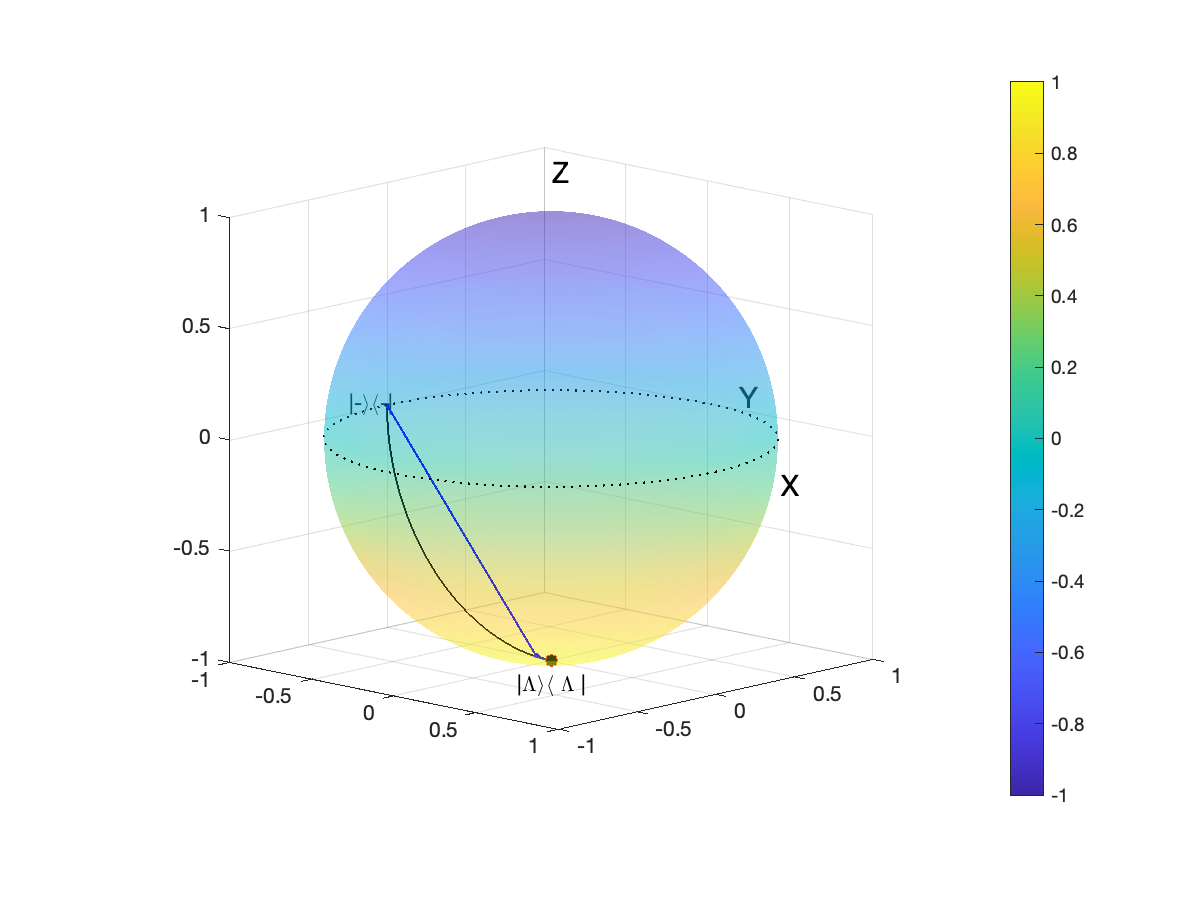
\includegraphics[width=0.6\textwidth]{images/1qubit_Z.eps} \label{ex1_e}}
%        \subfloat[Mixed State Trajectory]{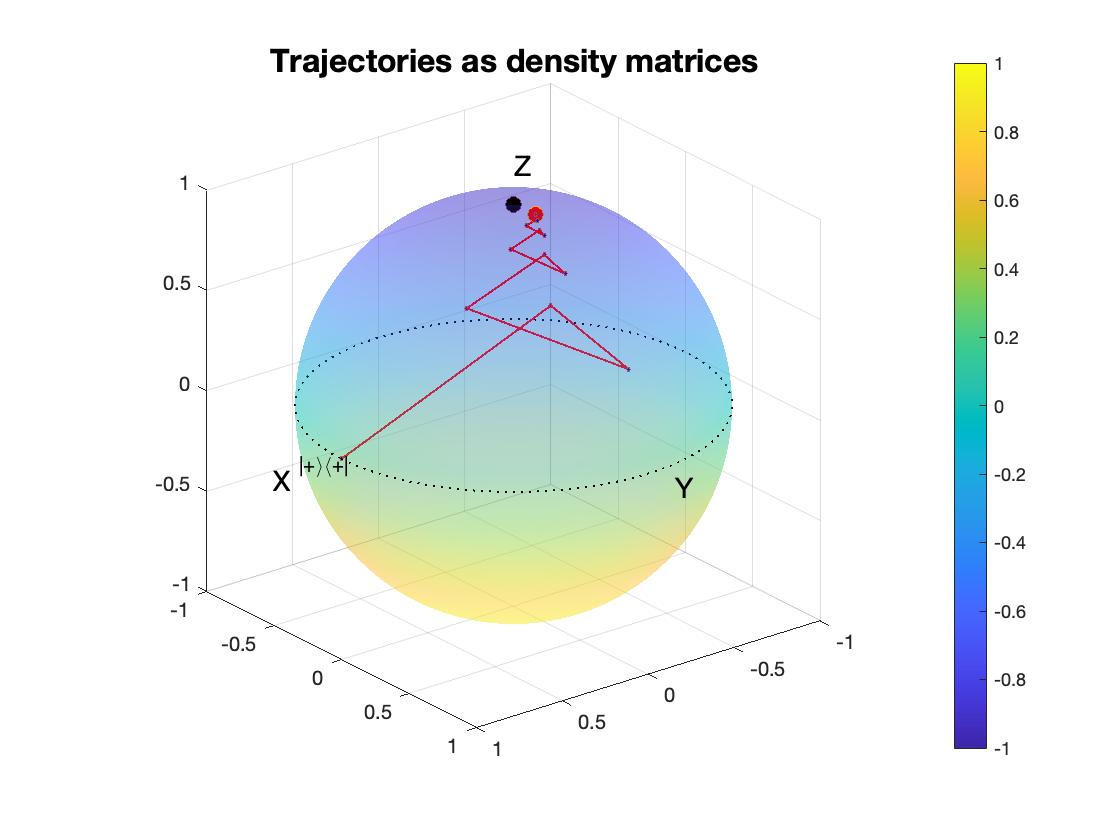
\includegraphics[width=0.5\textwidth]{images/1qubit_m.jpg} \label{ex1_e}}
        
    \caption{Example of the evolution of pure state (black line) and density matrix(blue line) with a single qubit}
    \label{fig:enter-label}
\end{figure}


% Plot showing decaing overlap with bad states and increasing overlap with good states over iterations (with varying values of B_z)

% Bloch picutres of pure/mixed states, 
% Initial state, Algorithm with Bz = 1, ... 0.1, Final state,  
% 100 runs, with pure states, and average them.



\subsection{Example 2: Many qubits}
% Plots showing decayig overlap with bad states and increasing overlap with good states over iterations
% Result showing preferential scaling with ancillas
% Plot of scaling with increasing number of qubits (for physical model)

% Start with \sum_i B X_i Z_{i+1} and show plots 
% f(n,m) = #iteration > 0.9, for each of m=1, m=ceil(log n), m = n; 

\begin{figure}[h]
    \centering
        \subfloat[Algorithm with m=2 ancillary qubits]{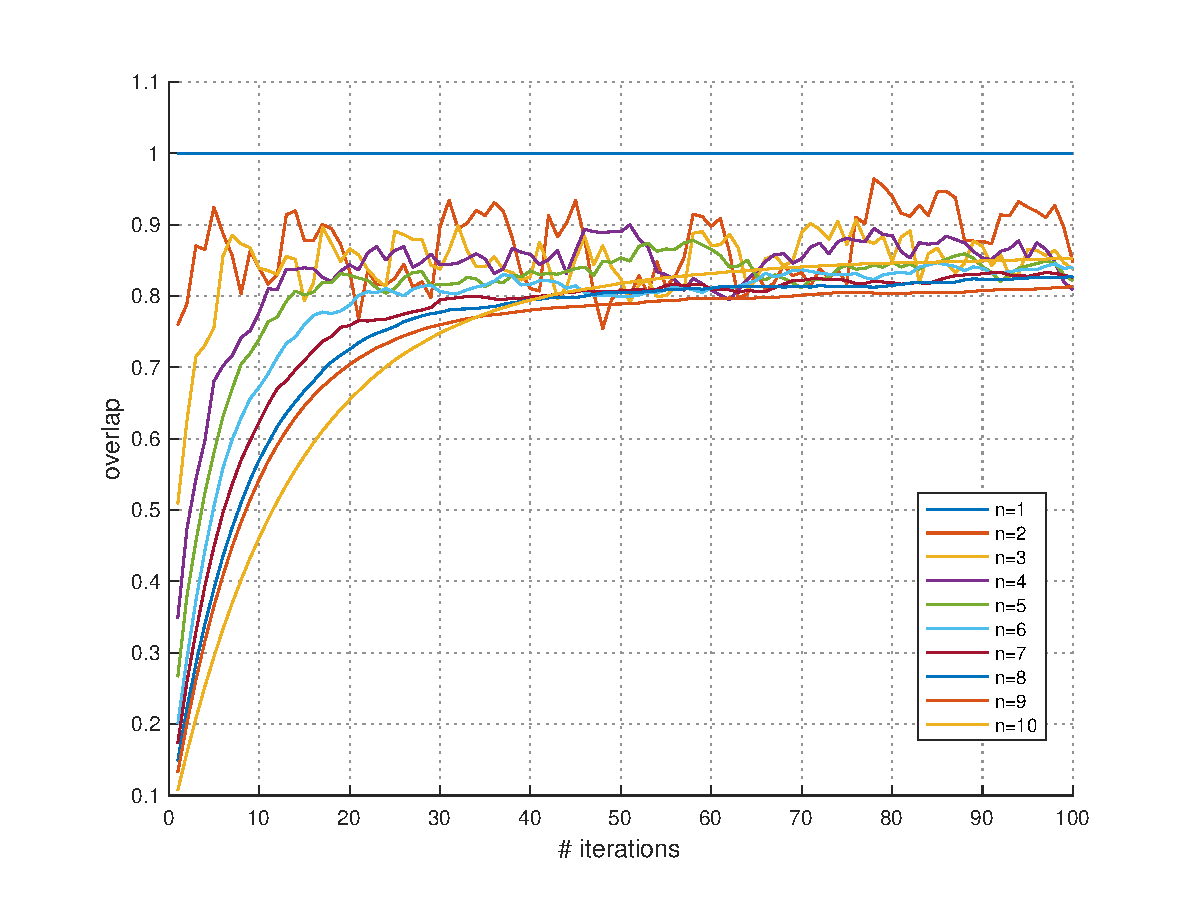
\includegraphics[width=0.5\textwidth]{images/Diag_runs.eps} \label{ex1_e}}
        \subfloat[Rate of Convergence]{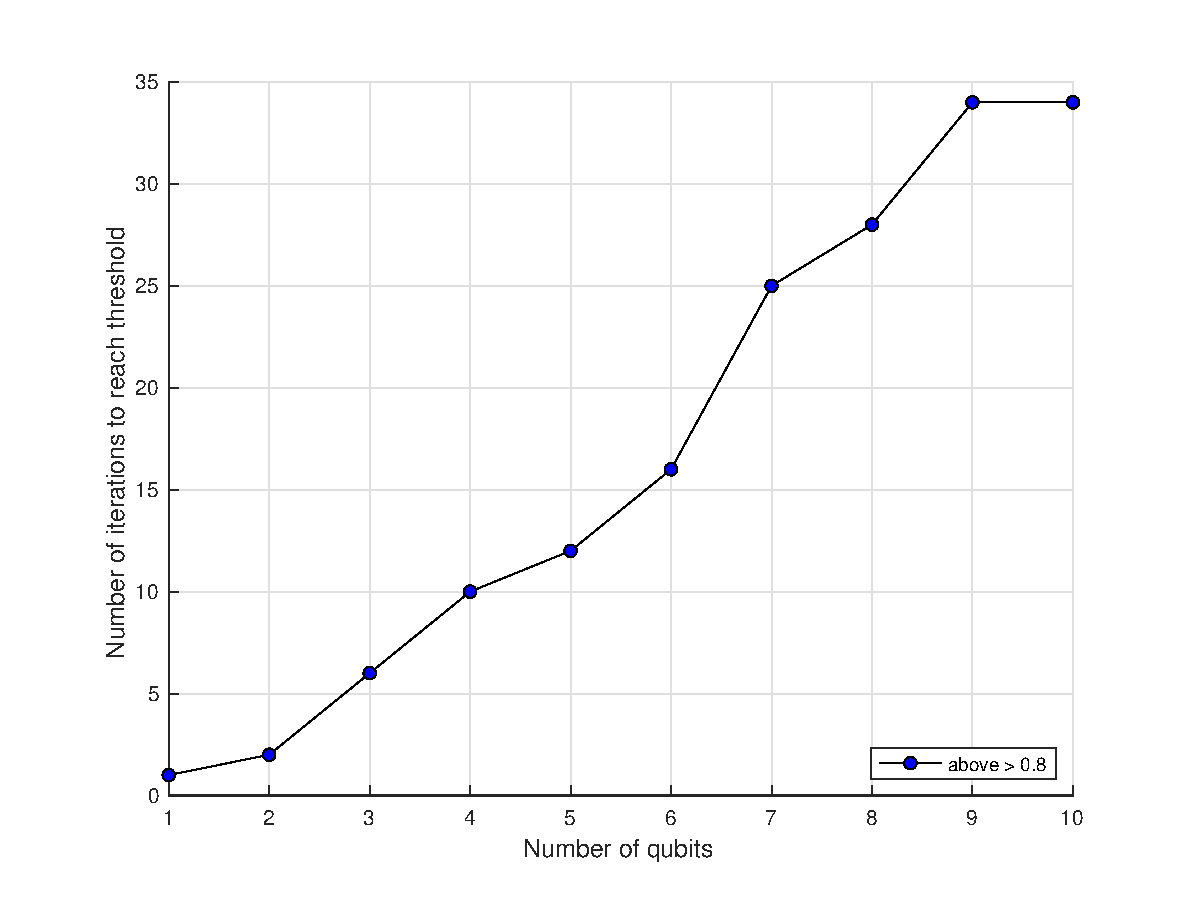
\includegraphics[width=0.5\textwidth]{images/Diag_rate_of_convergence.eps} \label{ex1_e}}
    \caption{The figures illustrate a typical rate of convergence of a normalised N-dimensional Diagonal matrix with uniform eigenvalues between $[N/2:N/2-1]$ for $n=log_2(N)$ taking values 1 to 10. The norm is $n^2$. $\Lambda_0=-\frac{1}{n}, \Lambda_1=n$. We use Clenshaw-Curtis quadrature with the Truncation boundary of 40, and 5000 roots of Chebyshev Polynomials. }
\end{figure}


%\subsection{Examples 3: IBM-Q}

%\section{Heuristics: Generalisation to constructing polygons filters}
%% There was a nice idea about generalising the rectangles to other other shapes with the idea that they might lead to faster convergence. 
% We could do some fun shapes here.

\section{Discussions}
Conjecture: For quantum dynamical systems on $n$ qubits, with norm atmost $poly(n)$, spanning a small $\sim O(n^2)$ dimensional lie algebra (such as Kitaev, XY, TFIM models), there exists choices of maps such that, under idealised conditions, the algorithm converges in poly($n$) iterations, when \\
(1) $|\Lambda1 - \Lambda_0| \geq \frac{1}{poly(n)}$.\\
(2) Density of states in interval $(\Lambda_0,\Lambda_1)$ is atleast $\frac{poly(n)}{2^n}$ 

In general the minimum number of applications of the map $r$ and the number of ancillary qubits $m$ required to prepare a microcanonical ensemble is bounded by $n$, and $n \leq m*r$ \cite{Z24}.

Sampling from microcanonical ensembles is as hard as preparing low energy states as one can lower bound the norm of a hamiltonian H and do a bisection search over different $\Lambda$ intervals to sample from a microcanonical ensemble of low energy states

Previous complexity theoretic studies on dissipative superoperators have studies have indicated there may be no significant advantage over unitary methods in the asymptotic settings. This work however reports progress on non-asymptotic settings.

%\appendix
\begin{appendix}
\begin{lemma}[Simplification of $e^{i\widetilde{H}^{\Lambda}_{\X}t} $]
\label{lemma_simplify_h}
Given $\widetilde{H}^{\Lambda}_{\X} = \sum_{j=1}^m \ket{1}\bra{0}_j \otimes P_{\Lambda}X_j + \ket{0}\bra{1}_j \otimes X_j^{\dagger} P_{\Lambda}$ where $P_{\Lambda}$ is a projector and $X_j$ are unitary matrices:
    \begin{multline*}
        e^{i\widetilde{H}^{\Lambda}_{\X}t} = \mathbb{I} + (\cos(t) -1)\sum_{j=1}^m (\ket{1}\bra{1}_j\otimes P_{\Lambda}+\ket{0}\bra{0}_j\otimes X_j^{\dagger}P_{\Lambda} X_j) +\\ i\sin(t)\sum_{j=1}^m(\ket{1}\bra{0}_j \otimes P_{\Lambda} X_j+\ket{0}\bra{1}_j \otimes  X_j^{\dagger}P_{\Lambda}))
    \end{multline*}
\end{lemma}
\begin{proof}
    Let us define the following operators:
    \begin{align*}
        A_j &= \ket{1}\bra{0}_j \otimes P_{\Lambda} X_j\\
        B_j &= \ket{1}\bra{1}_j\otimes P_{\Lambda}\\
        C_j &= \ket{0}\bra{0}_j\otimes X_j^{\dagger}P_{\Lambda} X_j
    \end{align*}
    Then as $X$ is unitary and $P_{\Lambda}$ is a projector the following relations hold:
    \begin{align*}
        A_iA_j^{\dagger} = B_j\delta_{ij}&, A_i^{\dagger}A_j = C_j\delta_{ij}\\
        B_iB_j = B_j\delta_{ij}, C_iC_j = C_j\delta_{ij}&, B_j= B_j^{\dagger}, C_j=C_j^{\dagger} \\
        B_iA_j = A_j\delta_{ij}&, A_iC_j = A_j\delta_{ij} \\
        A_iA_j = 0, B_iC_j = 0&,C_iA_j= 0, A_iB_j = 0
    \end{align*}
    Hence, $(A_j+A_j^{\dagger})^2 = B_j+C_j$, $(B_j+C_j)^n = B_j+C_j$ and $(B_j+C_j)(A_j+A_j^{\dagger}) = A_j+A_j^{\dagger}$, so:
    \begin{align}
    e^{i\widetilde{H}^{\Lambda}_{\X}t} = e^{i\sum_{j=1}^m(A_j+A_j^{\dagger})t} &= \prod_{j=1}^m\sum_{k=0}^{\infty} \frac{(it)^k}{k!} (A_j+A_j^{\dagger})^k \\
    &= \prod_{j=1}^m\bigg(\mathbb{I} + \sum_{k=1}^{\infty}\frac{(it)^{2k}}{(2k)!} (B_j+C_j) + \sum_{k=0}^{\infty}\frac{(it)^{2k+1}}{(2k+1)!} (A_j+A_j^{\dagger})\bigg)\\
    &= \prod_{j=1}^m\bigg(\mathbb{I} + (\cos(t) -1) (B_j+C_j) + i\sin(t)(A_j+A_j^{\dagger})\bigg)\\
    &= \mathbb{I} + (\cos(t) -1)\sum_{j=1}^m (B_j+C_j) + i\sin(t)\sum_{j=1}^m(A_j+A_j^{\dagger})
    \end{align}
\end{proof}
\end{appendix}
\end{document}